\documentclass[conference]{IEEEtran}
\IEEEoverridecommandlockouts
% The preceding line is only needed to identify funding in the first footnote. If that is unneeded, please comment it out.
\usepackage{cite}
\usepackage{amsmath,amssymb,amsfonts}
\usepackage{algorithmic}
\usepackage{graphicx}
\usepackage{textcomp}
\usepackage{xcolor}
\usepackage{float}
\def\BibTeX{{\rm B\kern-.05em{\sc i\kern-.025em b}\kern-.08em
    T\kern-.1667em\lower.7ex\hbox{E}\kern-.125emX}}
\begin{document}

\title{HOMEWOEK 2}

\author{\IEEEauthorblockN{Runlin Hou}
\IEEEauthorblockA{\textit{ECE, School Of Graduate Studies} \\
\textit{Rutgers University}\\
hourunlinxa@gmail.com}
}

\maketitle

\section*{problem 1}
The computational graph is shown as follow,
\begin{figure}[H]
    \centerline{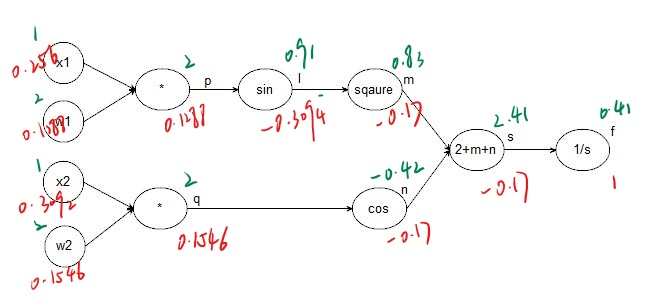
\includegraphics[scale=0.4]{pic1.jpg}}
    \caption{Computational Graph}
\end{figure}

And the derication is as follow:
\[\begin{aligned}
    \frac{df}{dx_1} &= -\frac{2w_1sin(w_1x_1)cos(w_1x_1)}{(2+sin^2(w_1x_1)+cos(w_2x_2))^2}\\
    \frac{df}{dw_1} &= -\frac{2x_1sin(w_1x_1)cos(w_1x_1)}{(2+sin^2(w_1x_1)+cos(w_2x_2))^2}\\
    \frac{df}{dx_2} &= \frac{w_2sin(w_2x_2)}{(2+sin^2(w_1x_1)+cos(w_2x_2))^2}\\
    \frac{df}{dw_2} &= \frac{x_2sin(w_2x_2)}{(2+sin^2(w_1x_1)+cos(w_2x_2))^2}
\end{aligned}\]

The result computed by program and above functions with input being $x=[1,1]$ $w=[2,2]$ are as follow, we can see that they are 
exactly the same.

\begin{figure}[H]
    \centerline{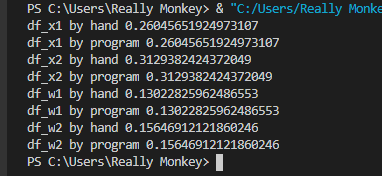
\includegraphics[scale=0.8]{pic2.png}}
    \caption{Program Result}
\end{figure}

\section*{problem 2}
The computational graph is shown as follow,
\begin{figure}[H]
    \centerline{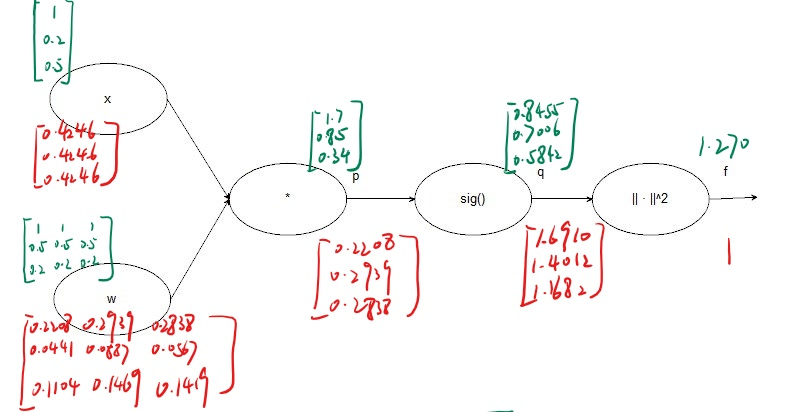
\includegraphics[scale=0.27]{pic3.jpg}}
    \caption{Computational Graph}
\end{figure}

The result from program is as follow. As we can see the results are the same as the above.
\begin{figure}[H]
    \centerline{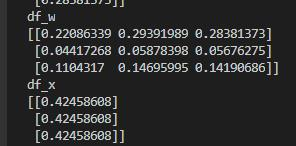
\includegraphics[scale=0.8]{pic4.jpg}}
    \caption{Computational Graph}
\end{figure}




\end{document}